This tool, as the \unix{} \emph{paste}, merges voices parallel to each other in the time
perspective. In other words, each individual voice will start at the beginning of the resulting
score.

Some decisions were made regarding what should be done with some information present in each tune.
This ensured that the resulting tune was consistent with each individual tune:

\begin{enumerate}
  \item The resulting tune's header derives from the first tune which has an actual tune written, in
  other words, at least one \emph{note}.
  \item The \context{} is updated every time a change is detected during the tune's traversal. It is
  a local data structure that comprises the \emph{current voice} and its \emph{key}, \emph{meter},
  \emph{length}, \emph{tempo} and \emph{number of measures}.
  \item Any \context{} change detected, like the \emph{key} or the \emph{meter}, is written to the
  resulting tune only if it is different from the current \context{}.
  \item In the resulting tune, any voice that has fewer measures than the longest one is appended
  with the necessary \measurerests{} to match the longest.
\end{enumerate}

\subsection*{Algorithm}

\pasteabc{}'s algorithm is divided in three stages: \textbf{1)} retrieving the header for the
resulting tune, \textbf{2)} pasting the tunes and \textbf{3)} appending any necessary
\measurerests{}. In the end, the output generated is printed to the output.

An algorithmic description is made in algorithm \ref{alg:pasteabc}.

\begin{enumerate}
\item As mentioned before, the resulting tune's header comes from the first tune with at least
one \emph{note} written.

This stage follows a simple algorithm where each tune is processed by \dt{} in the order they are
passed in. As soon as a tune with a \emph{note} written is found, it stops and returns that tune's
header. During the tune's traversal, the \context{} is updated. It will be used in the final stage
where a post processing is done to guarantee the resulting tune's validity.

The set of \abcdtrules{} to be passed to \dt{} consists in applying a blank transformation to every
\abcelement{} with state \intune{} or \inline{} (consult section \ref{sec:abcdt_rules} for more
information on state), activating a flag when a \emph{note} is found to stop processing further
tunes and, finally, recording the \context{}. See table \ref{tab:paste_fst_stg_rules} for a
description of the \abcdtrules{}.

\begin{center}
  \begin{table}[h]
    \begin{tabular}{|p{2.25cm}|p{7.25cm}|p{5cm}|}
      \hline
      Actuator & Transformation (Perl) & Notes\\
      \hline
      \hline
      \intune{} & q\{\}; &
      \\
      \hline

      \hline
      \inline{} & q\{\}; &
      \\
      \hline

      \hline
      \emph{note} & \$has\_tune = 1; q\{\}; &
      \\
      \hline

      \hline
      \inheader{}::\emph{M:} & update\_context(\{meter => 1\}); toabc(); & \emph{update\_context} is
      a local function that updates, in this rule's case, the \context{}'s meter. \toabc{} is called
      in the end so that the actual \abcelement{} is printed instead of the returning value from the
      previous statement.
      \\
      \hline

      \hline
      \inheader{}::\emph{L:} & update\_context(\{length => 1\}); toabc(); &
      \\
      \hline

      \hline
      \inheader{}::\emph{K:} & update\_context(\{key => 1\}); toabc(); &
      \\
      \hline

      \hline
      \inheader{}::\emph{Q:} & update\_context(\{tempo => 1\}); toabc(); &
      \\
      \hline
    \end{tabular}
    \caption{\abcdtrules{} for \pasteabc{}'s first stage}
    \label{tab:paste_fst_stg_rules}
  \end{table}
\end{center}

\item This stage's consists in processing each tune with \dt{} and concatenating each individual
result. This is the actual pasting where each tune's original \abc{} is returned except for the
following parts.

The header from each tune is not printed since it has already been retrieved in the previous stage.

abcMIDI commands \emph{\%\%staves} and \emph{\%\%score} are not printed as well, since each voice's
positioning on the resulting score may differ from the original one.

The \context{} is also being recorded each time one of its constituents is found, which enables the
possibility of not printing the context change if it is the same as the current one. This makes the
resulting tune cleaner without useless duplications. See table \ref{tab:paste_snd_stg_rules}.

\begin{center}
  \begin{table}[h]
    \begin{tabular}{|p{2.5cm}|p{4.75cm}|p{8cm}|}
      \hline
      Actuator & Transformation (Perl) & Notes\\
      \hline
      \hline
      \emph{in\_global::info} & q\{\}; &
      \\
      \hline

      \hline
      \emph{in\_header::info} & q\{\}; &
      \\
      \hline

      \hline
      \emph{staves} & q\{\}; &
      \\
      \hline

      \hline
      \emph{score} & q\{\}; &
      \\
      \hline

      \hline
      \emph{bar} & update\_measure\_count(); toabc(); & \emph{update\_measure\_count} is a local
      function that increments the measure count for the current voice.
      \\
      \hline

      \hline
      \emph{V:} & print\_voice(); & Local function that prints the voice element if it is different
      from the current voice. Also, if this voice has been previously defined, then the short form
      of the voice's \abcelement{} is printed. \context{}'s voice is updated.
      \\
      \hline

      \hline
      \emph{M:} & print\_meter(); & Local function that prints the meter element if it is different
      from the current meter. \context{}'s meter is updated.
      \\
      \hline

      \hline
      \emph{L:} & print\_length(); & Same as the previous rule but applied to the length element.
      \\
      \hline

      \hline
      \emph{K:} & print\_key(); & Same as the previous rule but applied to the key element.
      \\
      \hline

      \hline
      \emph{Q:} & print\_tempo(); & Same as the previous rule but applied to the tempo element.
      \\
      \hline

    \end{tabular}
    \caption{\abcdtrules{} for \pasteabc{}'s second stage}
    \label{tab:paste_snd_stg_rules}
  \end{table}
\end{center}

\item The final step consists in verifying if there is any voice with fewer measures than the voice
with the biggest number of measures. If there is such a voice then a \measurerest{} with length
equal to the missing measures is appended after that voice. This is possible because, in step
\textbf{2)}, the number of measures for each voice was being recorded.
\end{enumerate}

\begin{algorithm}[h]
  \KwIn{abc\_tunes}
  \ForAll{$ tune \in abc\_tunes $}{
    $header \gets dt(tune,$ rules from table \ref{tab:paste_fst_stg_rules}$)$ \hfill //1)\\
  }
  \ForAll{$ tune \in abc\_tunes $}{
    $res \gets res$ ++ $dt(tune,$ rules from table \ref{tab:paste_snd_stg_rules}$)$ \hfill //2)\\
  }
  $measures \gets add\_measures()$ \hfill //3)\\
  \Return{$header$ ++ $res$ ++ $measures$}
  \caption{\pasteabc{}'s algorithm}
  \label{alg:pasteabc}
\end{algorithm}

\subsection*{Usage}

Listing \ref{lst:pasteabcman} shows \pasteabc{}'s manual.\\

\lstinputlisting[caption={\pasteabc{}'s manual},label={lst:pasteabcman},captionpos=t,abovecaptionskip=-\medskipamount,float]{misc/paste_manual.tex}

Listing \ref{lst:paste_abc_by_example} shows a usage example for \pasteabc{}. It reads tunes
\textbf{101.abc} (listing \ref{lst:verbum_s1_p1}) and \textbf{103.abc} (listing
\ref{lst:verbum_s1_p3}) and its output is shown in listing \ref{lst:verbum_s1_p1_p3_pasted} along
with the corresponding score (figure \ref{fig:verbum_s1_p1_p3_score}).\\

\begin{lstlisting}[caption={\pasteabc{} by example},label={lst:paste_abc_by_example},captionpos=t,abovecaptionskip=-\medskipamount]
paste_abc 101.abc 103.abc
\end{lstlisting}

\lstinputlisting[caption={Verbum caro factum est: Section 1; Part 1 - Soprano},label={lst:verbum_s1_p1},captionpos=t,abovecaptionskip=-\medskipamount]{misc/verbum_s1_p1.tex}

\vspace{-0.25cm}
\begin{figure}[H]
  \begin{center}
    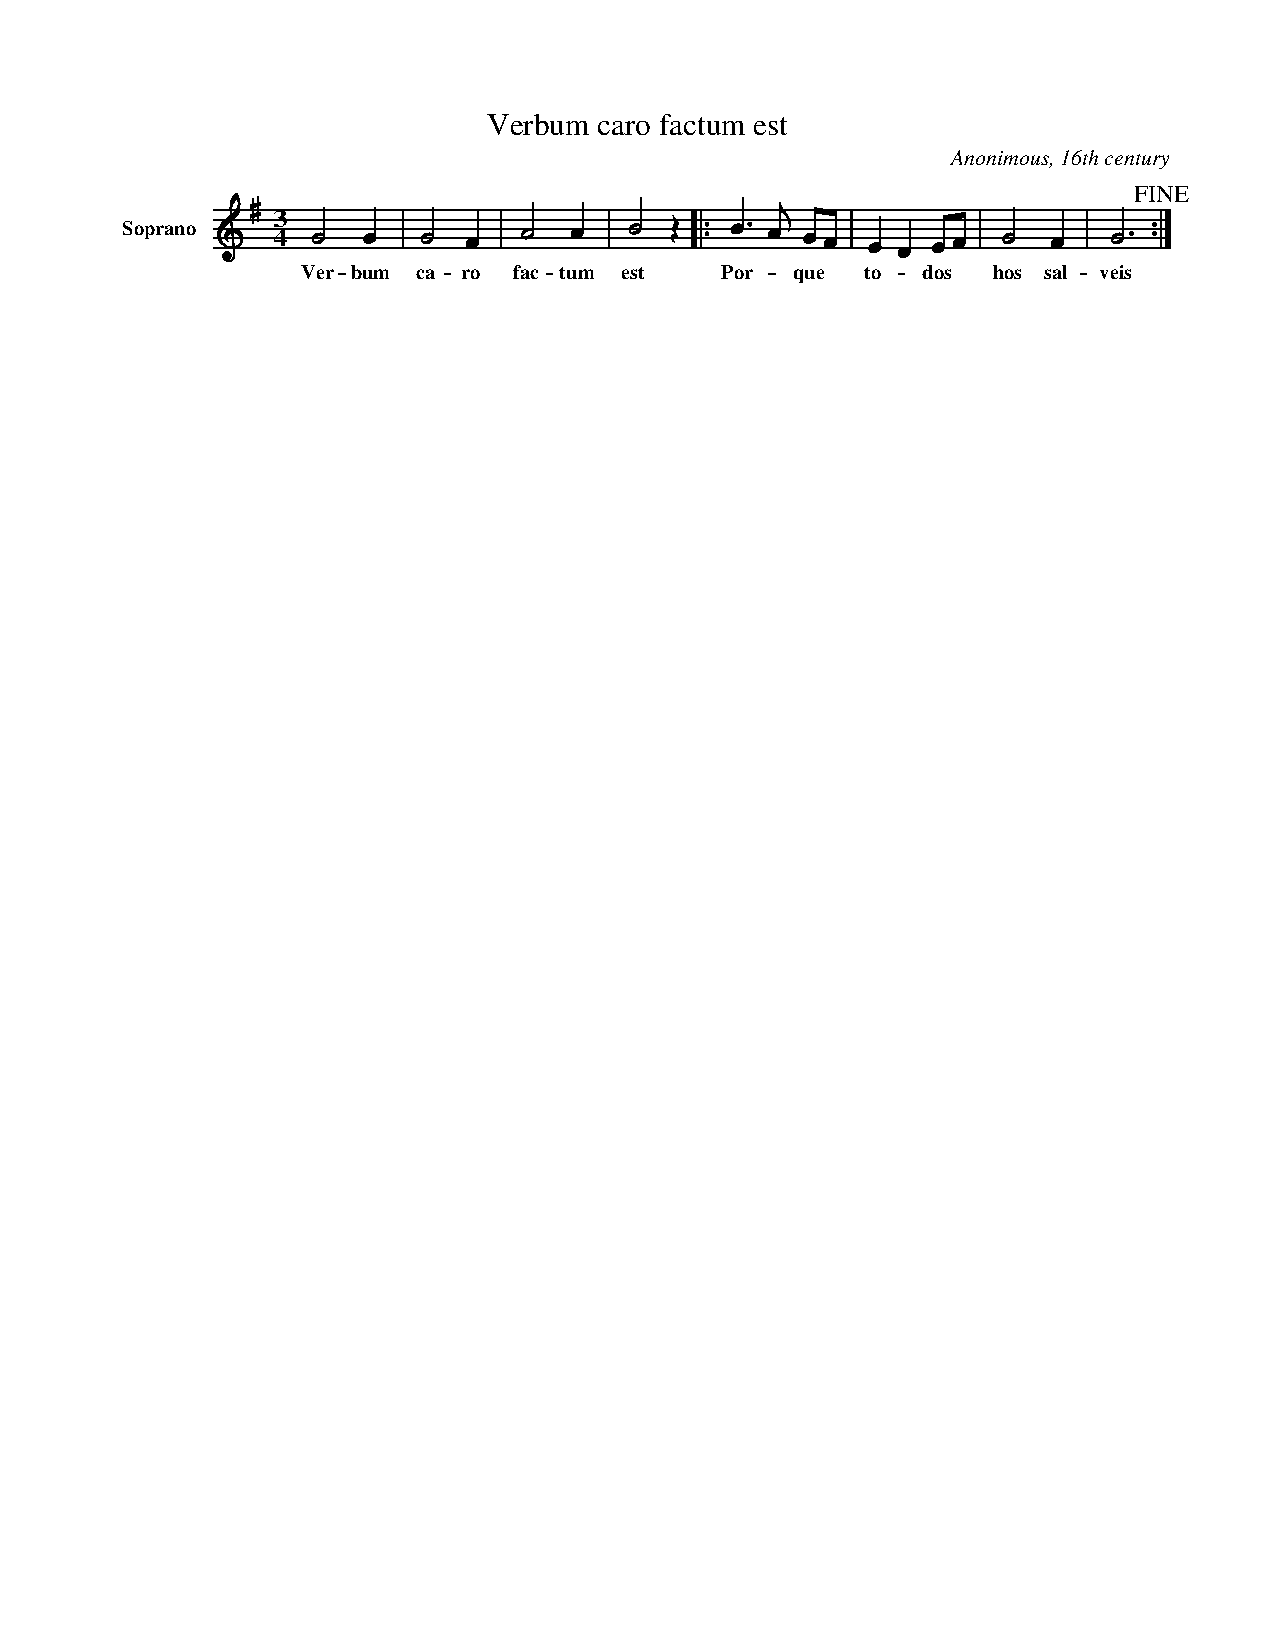
\includegraphics[width=0.8\textwidth, clip=true, trim = 0mm 230mm 0mm 17mm]{img/101.pdf}
    \caption{Verbum caro factum est: Section 1; Part 1 - Soprano (Score)}
    \label{fig:verbum_s1_p1_score}
  \end{center}
\end{figure}

\lstinputlisting[caption={Verbum caro factum est: Section 1; Part 3 - Tenor},label={lst:verbum_s1_p3},captionpos=t,abovecaptionskip=-\medskipamount]{misc/103.tex}

\vspace{-1.30cm}
\begin{figure}[h]
  \begin{center}
    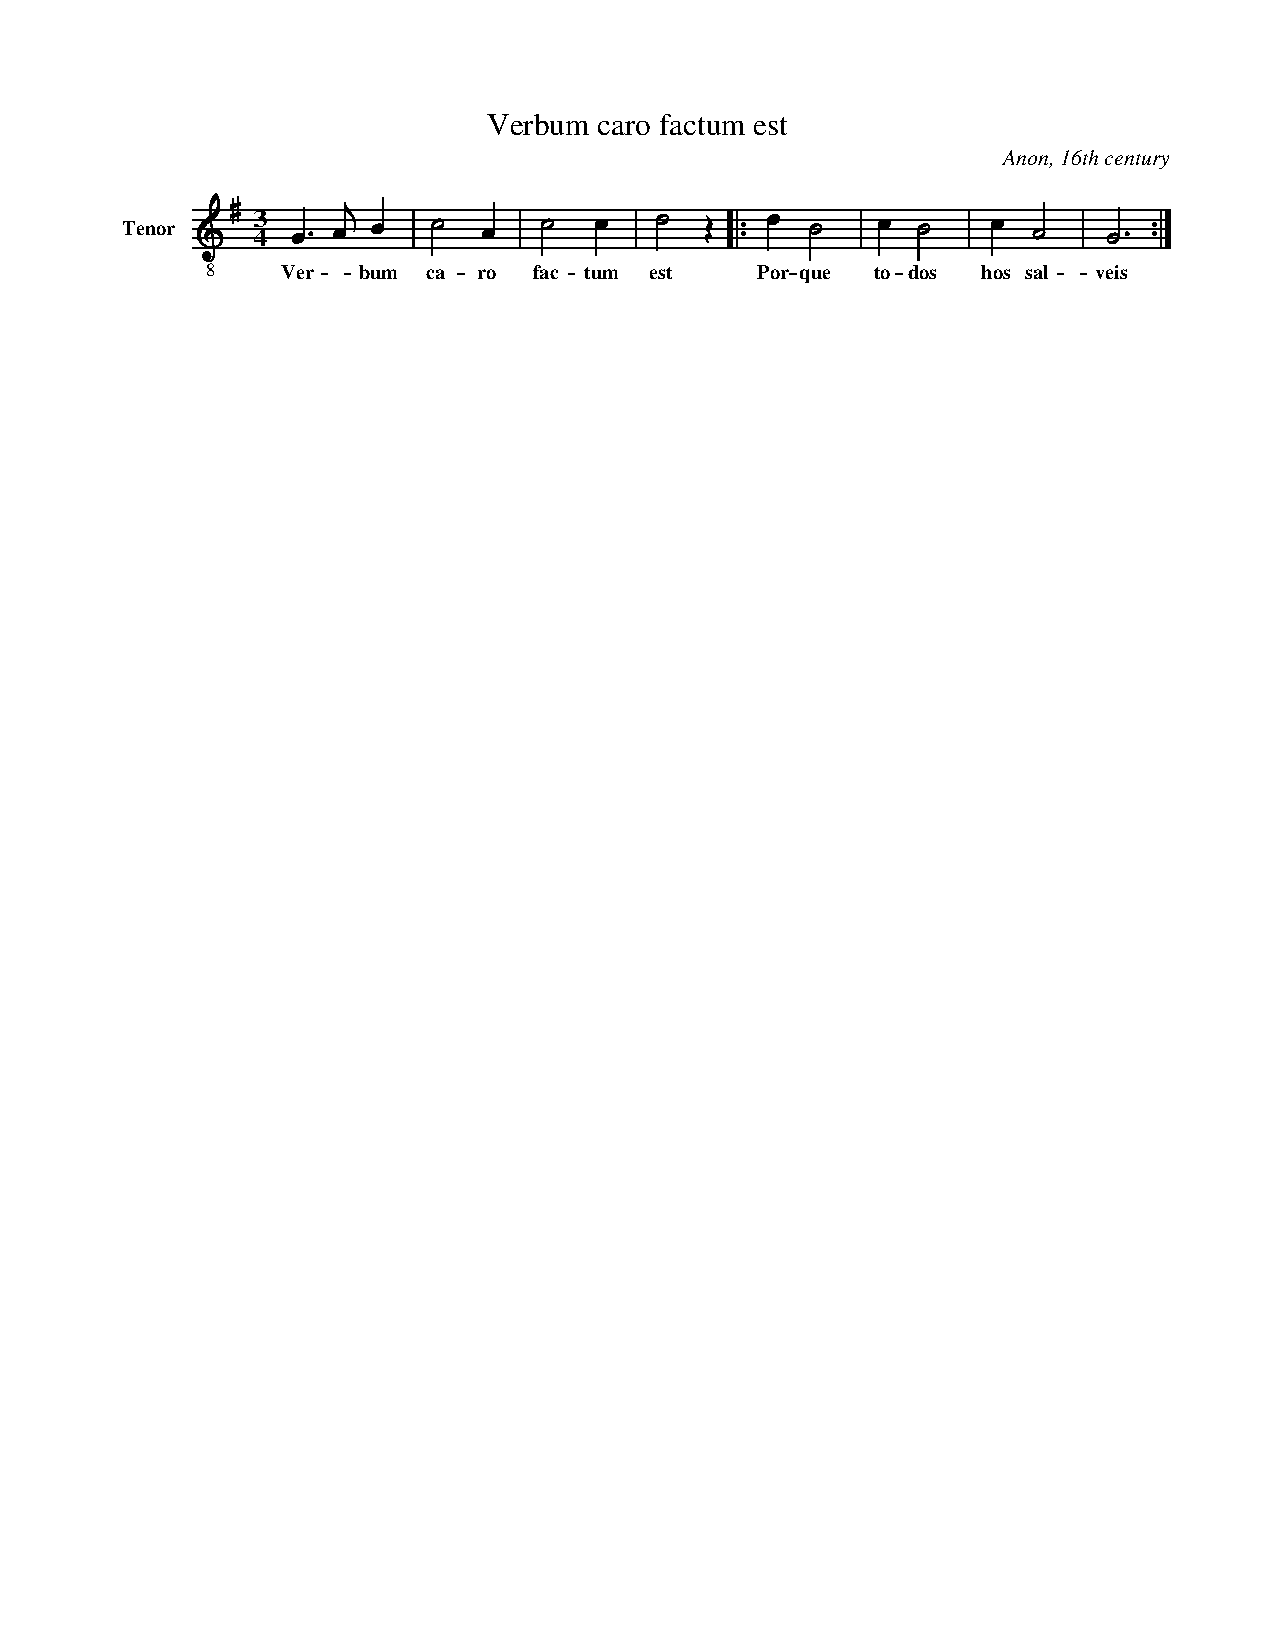
\includegraphics[width=0.8\textwidth, clip=true, trim = 15mm 231mm 17mm 0mm]{img/103.pdf}
    \caption{Verbum caro factum est: Section 1; Part 3 - Tenor (Score)}
  \end{center}
\end{figure}

\lstinputlisting[caption={Verbum caro factum est: Section 1; Part 1 \& 3},label={lst:verbum_s1_p1_p3_pasted},captionpos=t,abovecaptionskip=-\medskipamount]{misc/verbum_s1_p1_p3_pasted.tex}

\vspace{-1.30cm}
\begin{figure}[h]
  \begin{center}
    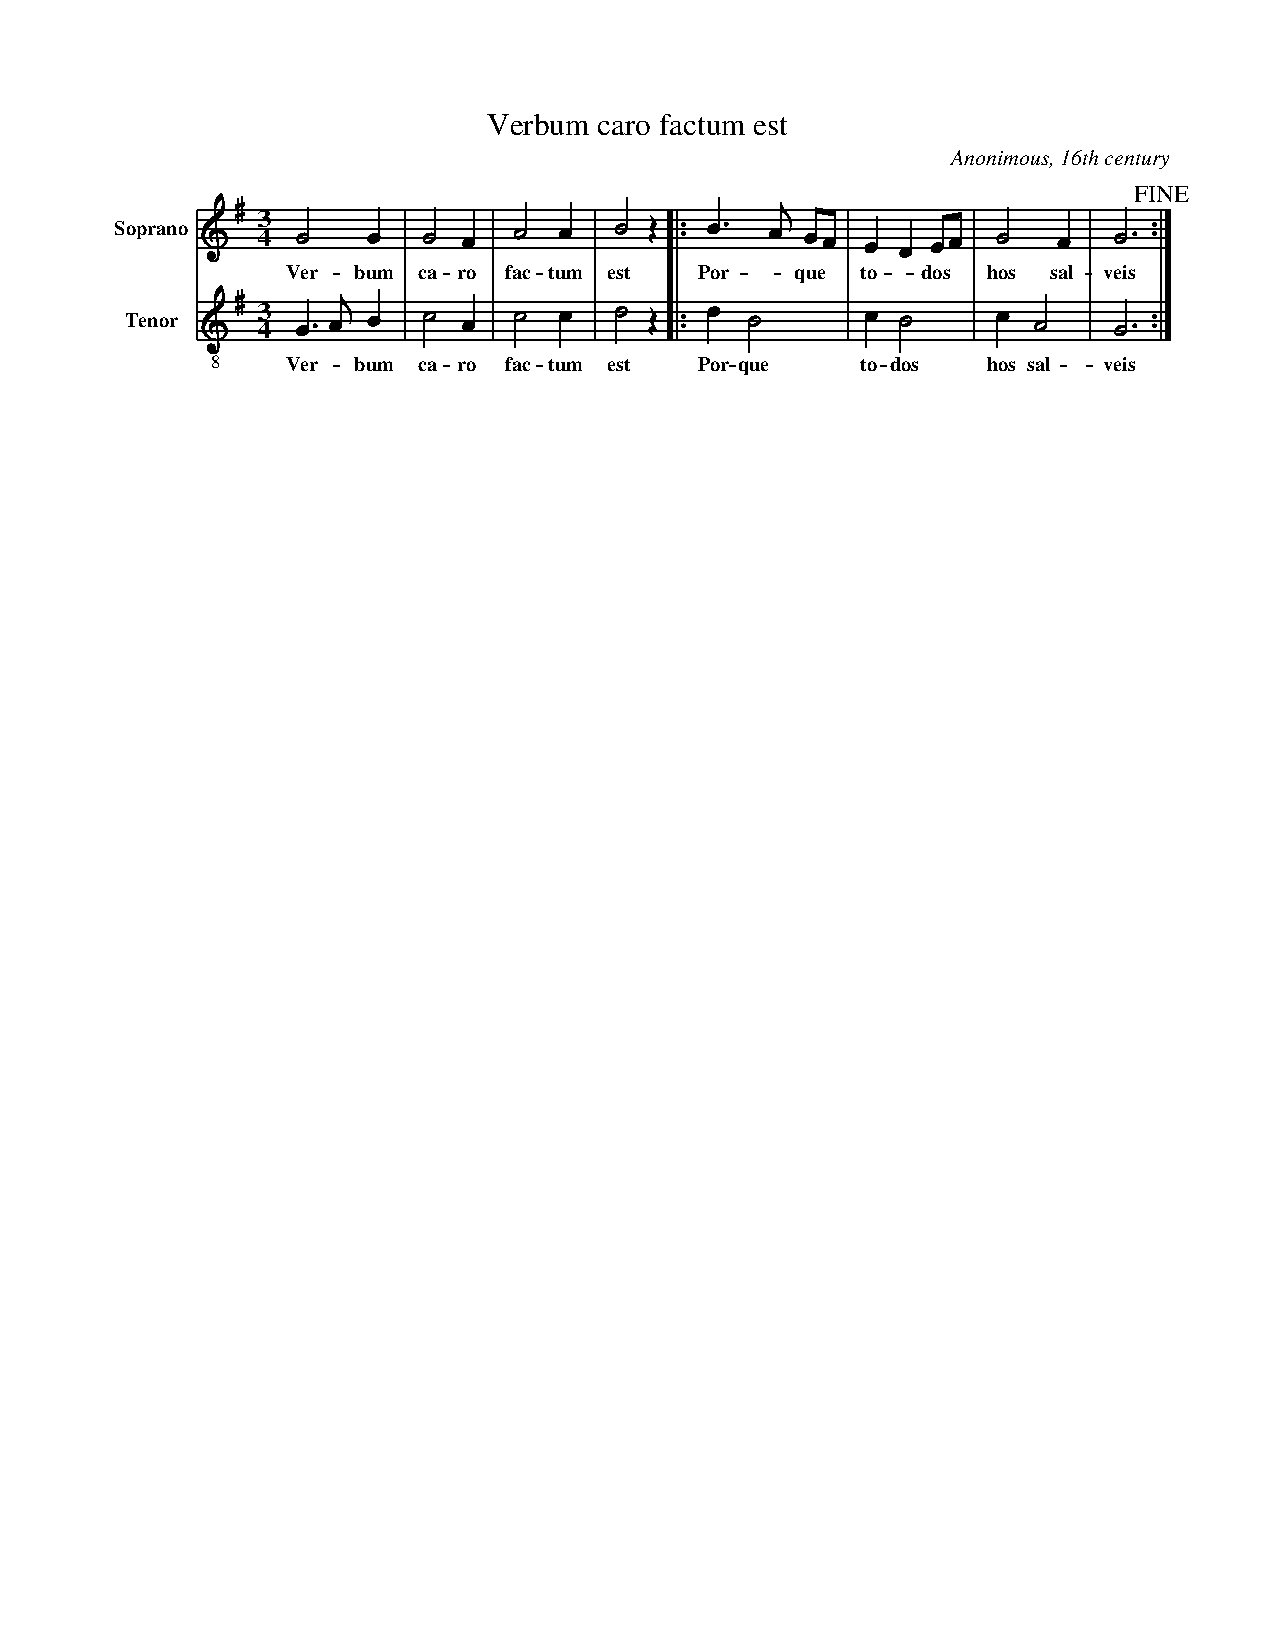
\includegraphics[width=0.8\textwidth, clip=true, trim = 15mm 210mm 15mm 0mm]{img/verbum_s1_p1_p3.pdf}
    \caption{Verbum caro factum est: Section 1; Part 1 \& 3 (Score)}
    \label{fig:verbum_s1_p1_p3_score}
  \end{center}
\end{figure}
